\documentclass{article}

\usepackage{pgfplots} %http://www.ctan.org/pkg/pgfplots
\pgfplotsset{compat=newest, set layers=standard}


\usepgfplotslibrary{fillbetween}
\usetikzlibrary{intersections}
\begin{document}
\begin{figure}

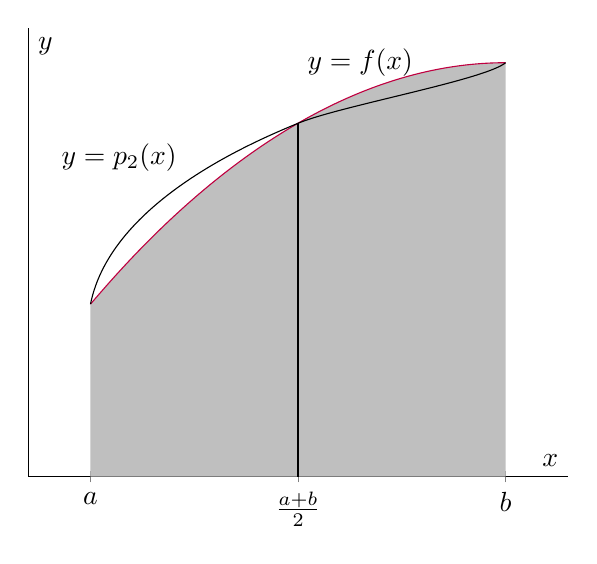
\begin{tikzpicture}
\begin{axis}[axis lines=center, ytick=\empty, 
ymax=1.3, ymin=0, xmax=2.6,xmin=0,
xtick={0.3,1.3,2.3}, xticklabels={$a$,$\frac{a+b}{2}$,$b$},
axis line style={-}, xlabel=$x$, ylabel=$y$]
\draw[name path=A, purple] (2.3,1.2) parabola (0.3,0.5);
\node[] at (1.6,1.2){$y=f(x)$};
\path[name path=B] (\pgfkeysvalueof{/pgfplots/xmin},0) 
                   --(\pgfkeysvalueof{/pgfplots/xmax},0);
\addplot[gray!50] fill between[of=A and B,soft clip={domain=0.3:2.3}];
\draw[name path=C] (1.3,0) -- (1.3,1.025);
\path[name intersections={of=A and C}] coordinate (midpoint) at (intersection-1);
\draw (0.3,0.5) ..controls ++(0.1,0.3) and ++(-0.2,-0.05) .. (midpoint)
                node[pos=0.5,above left]{$y=p_2(x)$} 
                ..controls ++(0.2,0.05) and ++(-0.1,-0.05) .. (2.3,1.2);
\end{axis}
\end{tikzpicture}

$h = \frac{b-a}{2}$

$$\int_a^b f(x)dx \approx \frac{h}{3} \sum_{k=1}^{N/2} \{f(x_{2k-2})+4f(x_{2k-1})+f(x_{2k}))\}$$


\end{figure}

\end{document}